\section{写优化索引}

\subsection{日志结构合并(LSM)树}

\begin{figure}[H]
    \centering
    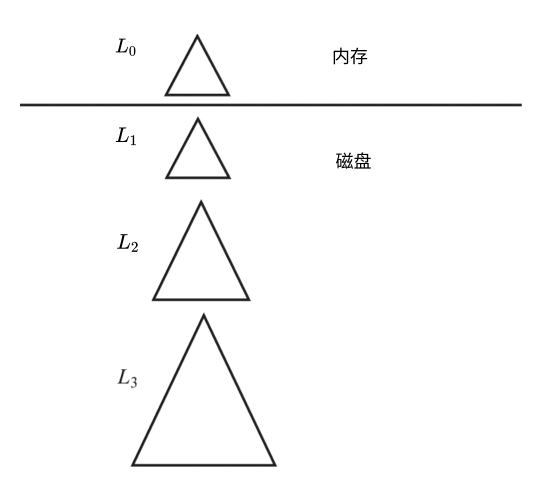
\includegraphics[width=0.9\linewidth]{image6.png}
    \caption{LSM树}
    \label{}
\end{figure}

\subsubsection{什么是LSM树}

LSM树是一种专门为 高吞吐量写入 优化的索引结构,常用于需要频繁插入(insert)和查询(query)的场景,尤其对 磁盘或闪存(SSD/Flash) 后端极为友好。其核心思想是:

\begin{enumerate}
    \item 写请求先写到内存中的小结构(MemTable),避免磁盘小量随机写。
    \item 当内存结构满后,以 批量顺序写 的方式「刷新」(flush)到磁盘上的一个较小层次。
    \item 随后当磁盘上该层数据积累到一定阈值,再与下一级更大的层次进行“合并”(merge),形成更大规模的有序文件。
    \item 通过多级、批量、顺序 I/O(而非随机写),显著减少磁盘写入的开销。
\end{enumerate}

$L_0$:维护一个 “可排序的内存结构”(通常是跳表、红黑树或MemTable),写速度非常快。

$L_1,L_2,...$(磁盘):每一层都是一个或多个 “有序文件” 或 “B+树结构”,它们依次满足“容量逐层增大”的策略。

当$L_0$满时,会以批量方式将数据合并到$L_1$;当$L_1$达到阈值时,再和$L_2$做合并,以此类推。每次合并都是“顺序读旧数据 + 顺序写新数据”,大幅度减少对磁盘的随机写操作。

\subsubsection{LSM树的层次结构与阈值策略}

假设我们将$L_0$看作内存树,$L_1,L_2,L_3,...$都是磁盘上的有序结构(例如某种底层可拆分的SSTable或多路归并后生成的B+树文件),并且通常约定:

\begin{itemize}
    \item $L_0$的容量比较小,例如$C_0$个键后就出发flush
    \item $L_1$的容量上限为$C_1=k\times C_0$个键
    \item $L_2$的容量上限为$C_2=k\times C_1=k^2\times C_0$
    \item 以此类推:$C_{i+1}=k\times C_i$,其中$k$是一个常数
\end{itemize}

因此,当$L_0$内存结构积累到$C_0$键时,就会“批量写”到磁盘$L_1$;当$L_1$上积累到$C_1$键时,就会和$L_2$做一次更大批量的merge,生成新的$L_2$文件;以此类推。

这种逐层 “分级合并(tiered merging)” 或 “大小归并(size-tiered compaction)” 的方式正是LSM树的核心。

\subsubsection{INSERT流程}

下面用一段文字示例来说明 LSM 树插入的具体过程,以便对比其与传统 B+树的不同之处。

假设我们当前的各层状态如下:

内存层$L_0$还没有满,已存在若干键:$L_0:[<a,1>,<b,2>,<d,4>]$(以跳表或红黑树形式存储,因此是有序的)

磁盘层$L_1$现有一个有序文件(SSTable或B+树文件)包含键:$L_1:[<e,5>,<h,8>]$

磁盘层$L_2$为空或容量尚未到达阈值。

\noindent 1.写入"<c,3>":将其插入到内存层$L_0$。$L_0:[<a,1>,<b,2>,<c,3>,<d,4>]$。此时$L_0$键数=4.假设$C_0=4$(达到内存阈值),需要flush $L_0$到$L_1$.

\noindent 2.将$L_0$ flush到$L_1$: 

步骤2.1:先把$L_0$中所有键“顺序写”到磁盘,形成一个临时有序文件(SSTable),比如我们得到一个文件$F_0$包含:$F_0:[<a,1>,<b,2>,<c,3>,<d,4>]$

步骤2.2:将现有的$L_1$文件$[<e,5>,<h,8>]$与新生成的$F_0$做多路归并,得到新的$L_1$(容量$C_1=10$例如)。多路归并后:$L_1'=[<a,1>,<b,2>,<c,3>,<d,4>,<e,5>,<h,8>]$

步骤2.3:清空内存层$L_0$(再建一个空的跳表,让应用继续写)。

\noindent 3.持续插入并触发$L_1\to L_2$合并:后续若插入$<f,6>,<g,7>,<i,9>...$均进入$L_0$,直到$L_0$满再flush,当$L_1$中
键数累计到达阈值$C_1$(假设为6)时,就要触发$L_1$与$L_2$合并:

先将$L_1$当前文件(如[a,b,c,d,e,h])与最新的$L_1$ flush结果做归并,生成更大的一个临时文件。

归并后得到新的$L_2$文件(容量$C_2=k\times C_1$,例如60)

此后,清空$L_1$(或保留少量增量,以“分层归并”而不是“一次性全量归并”),保持$L_2$总是有序的。

\subsubsection{QUERY操作流程}

当我们要查询某个键(Key="X")时,LSM树必须分层搜索:

1.先到$L_0$(内存层)中查找。如果在这儿找到了 “<X, value>” 且没有 tombstone(删除标记),直接返回结果。

2.如果$L_0$中没有,再去$l_1$(最上层磁盘)查找;

3.若$L_1$中也没有,再去$L_2,L_3,...$依次查找。

4.如果在某一层发现了“删除标记(tombstone)”条目,则说明该 Key 已被删除,即使在更低层存在旧值,也当作“已删除”而返回空。

由于查询要向下搜索多层,会产生一定的查询延迟。但为了缩短查询路径,可以在每个层的文件中维护一个 布隆过滤器(Bloom Filter),先检查布隆过滤器,看该Key是否“可能存在”再决定是否真正读磁盘。这样可以避免绝大多数无意义的盘上查找。

\subsubsection{DELETE与UPDATE操作}

LSM 树中的删除与更新并不直接在磁盘层做随机删除,而是通过 “打墓碑(tombstone)” 的方式:

\noindent 1.DELETE:

\begin{itemize}
    \item 当应用请求删除某个键<X>时,首先向$L_0$(内存)中插入一条特殊的“删除条目”(tombstone),格式可以是<X, DELETE\_MARK>。
    \item 后续的查询如果先在$L_0$发现了<X, DELETE>,就判定为已删除,不往下层查旧值;
    \item 当$L_0$ flush到$L_1$时,这个tombstone也会连同正常条目一并合并。若在更低层$(L_1,L_2)$存在旧的<X,old\_value>,则在归并过程中一旦发现delete entry,就将对应的旧值直接过滤掉,保留delete tombstone;
    \item 如果tombstone也在更下层归并时被清理(因为它本身同样过时或者到了更低层合并时过期),就从索引中彻底删除该键。
\end{itemize}

\noindent 2.UPDATE:

更新其实等同于一次“删除旧值 + 插入新值”两个步骤:

1.向$L_0$插入<X,DELETE>标记(将旧值逻辑删除);

2.再向$L_0$插入<X,new\_value>(像正常插入一样排序);

在后续的归并过程中,归并算法会发现“先有 delete tombstone,再有新值”,则保留最新 <X, new\_value> 同时丢弃 tombstone;如果是相反次序,也会丢弃 tombstone并保留最新值。

\subsubsection{LSM 树的优缺点}

\noindent 优点

\begin{enumerate}
    \item 写入仅做顺序 I/O:不像B+树那样会频繁产生随机写,LSM树只会“先写内存,再批量顺序写磁盘”,有效减少磁盘写开销。
    \item 磁盘层文件始终满载:每次都进行合并,使得最终持久化到磁盘的文件几乎都是满页,避免空洞和空间浪费。
    \item 插入/删除吞吐量高:由于大多数插入都集中在内存,再通过合并在后台清理陈旧或删除条目,插入性能相比传统B+树更优。
\end{enumerate}

\noindent 缺点:

\begin{enumerate}
    \item 查询需要同时在多层查找:最坏情况下要查到最底层,如果每层都在磁盘上,就会导致多次随机读,查询延迟增加。可以通过 布隆过滤器(Bloom Filter) 降低多层查找次数(如果 Bloom Filter 判定不存在,就不去对应层做实际查找)。
    \item 数据被重复复制:每一次合并,都会把整层数据读出然后写入到下一层,导致重复 I/O。虽然是顺序I/O,但如果合并频繁,仍会带来开销。
\end{enumerate}

\subsubsection{Stepped-Merge Index(分级归并变种)}

为了进一步 降低磁盘写成本,有时会在每一层 不是只保留一个有序文件,而是保留 多个 (SSTable) 文件,形成 “分步合并(stepped-merge)” 的策略:

\begin{itemize}
    \item 每一层$L_i$允许存在最多$T_i$个小文件(SSTable)。
    \item 当超出阈值时,不是一次性把$L_i$所有文件合并到$L_{i+1}$,而是先将$L_i$中几个文件有选择地合并成一个新文件,放回$L_i$本层;
    \item 这样可以 减少每层向下合并的 I/O 规模,但查询时就要在更多文件中定位某个 Key,需要额外索引或 Bloom Filter 来过滤文件。
\end{itemize}

许多大数据存储系统(如 Google Bigtable、Apache Cassandra、MongoDB、LevelDB、MyRocks 等)都使用了这种 多文件分级合并 变种。

\subsection{缓冲树}

LSM树的替代方案。

核心思想:B+树的每个内部节点都有一个用于存储插入操作的缓冲区:当缓冲区满时,插入操作会被移到更低层次;若缓冲区较大,每次会有许多记录被移到更低层次;相应的,每条记录的I/O操作减少。

优势:查询开销更小,可与任何树索引结构一起使用。

缺点:比LSM树有更多随机I/O。